\documentclass[12pt]{article} 

%?? paths
\newcommand{\CiteMathPackage}{math} 
% \newcommand{\CiteReference}{reference.bib}

%?? packages 
\usepackage{setspace,geometry,fancyvrb,rotating} 
\usepackage{marginnote,datetime,enumitem} 
\usepackage{titlesec,indentfirst} 
\usepackage{amsmath,amsfonts,amssymb,amsthm,mathtools} 
\usepackage{threeparttable,booktabs,adjustbox} 
\usepackage{graphicx,epstopdf,float,soul,subfig} 
\usepackage[toc,page]{appendix} 
\usdate

%?? page setup 
\geometry{scale=0.8} 
\titleformat{\paragraph}[runin]{\itshape}{}{}{}[.] 
\titlelabel{\thetitle.\;} 
\setlength{\parindent}{10pt} 
\setlength{\parskip}{10pt} 
\usepackage{Alegreya} 
\usepackage[T1]{fontenc}

%?? bibliography 
\usepackage{natbib,fancybox,url,xcolor} 
\definecolor{MyBlue}{rgb}{0,0.2,0.6} 
\definecolor{MyRed}{rgb}{0.4,0,0.1} 
\definecolor{MyGreen}{rgb}{0,0.4,0} 
\definecolor{MyPink}{HTML}{E50379} 
\definecolor{MyOrange}{HTML}{CC5500} 
\definecolor{MyPurple}{HTML}{BF40BF}
\newcommand{\highlightR}[1]{{\emph{\color{MyRed}{#1}}}} 
\newcommand{\highlightB}[1]{{\emph{\color{MyBlue}{#1}}}} 
\newcommand{\highlightP}[1]{{\emph{\color{MyPink}{#1}}}} 
\newcommand{\highlightO}[1]{{\emph{\color{MyOrange}{#1}}}}
\newcommand{\highlightPP}[1]{{\emph{\color{MyPurple}{#1}}}}
\usepackage[bookmarks=true,bookmarksnumbered=true,colorlinks=true,linkcolor=MyBlue,citecolor=MyRed,filecolor=MyBlue,urlcolor=MyGreen]{hyperref} \bibliographystyle{econ}

%?? math and theorem environment 
\theoremstyle{definition} 
\newtheorem{assumption}{Assumption} 
\newtheorem{definition}{Definition} 
\newtheorem{theorem}{Theorem} 
\newtheorem{proposition}{Proposition} 
\newtheorem{lemma}{Lemma} 
\newtheorem{example}{Example} 
\newtheorem{corollary}[theorem]{Corollary} 
\usepackage{mathtools} 
\usepackage{\CiteMathPackage}

\begin{document} 

%??%??%??%??%??%??%??%??%??%??%??%??%??%??%??%??%??%??%??%??%??%?? 
%?? title 
%??%??%??%??%??%??%??%??%??%??%??%??%??%??%??%??%??%??%??%??%??%??

\title{\bf Coding Tests} 
\author{Wenzhi Wang} 
\date{\today} 
\maketitle 

A Github repository \href{https://github.com/wenzhi-econ/CodingTests}{(link here)} is created to store codes and summary report for the coding tasks. 

%??%??%??%??%??%??%??%??%??%??%??%??%??%??%??%??%??%??%??%??%??%?? 
%?? question 1 
%??%??%??%??%??%??%??%??%??%??%??%??%??%??%??%??%??%??%??%??%??%??

\section{Question 1: Simulations}

To present the results in a more simplified and unified way, from questions 1.1. to questions 1.4., I create a Python class that is able to conduct all the procedures required in the task. The complete codes are presented in Appendix Figure \ref{Codes_class}, and are stored in the ``codes/Question1.py'' script file.

The $\mathtt{ExpDistSimulation}$ class has three key attributes: $\mathtt{lambda\_value}$, $\mathtt{n\_sample}$, and $\mathtt{n\_simulation}$, which represents the distribution parameter of the exponential distribution, the sample size in each simulation, and the number of simulations, respectively. It has the following key methods and perform procedures required in the coding tasks:
\begin{itemize}[topsep=0pt, leftmargin=20pt, itemsep=0pt]
\setlength{\parskip}{10pt} 
\item $\mathtt{gen\_exp\_sample}$ generates a random draw from an exponential distribution (with default randomization seed 1234).
\item $\mathtt{cal\_sample\_mean}$ calculates the (unadjusted) sample mean from any random draw.
\item $\mathtt{adj\_sample\_mean}$ calculates the adjusted sample mean from any random draw.
\item $\mathtt{simulation}$ conducts simulation, and for each simulated sample, it calculates the adjusted sample mean and stores it.
\item $\mathtt{simulation\_plot}$ plots the empirical distribution of the simulated adjusted sample mean.
\end{itemize}

\newpage
\subsection{Question 1.1.}

First, I initialize different object instances with different sample size parameters. Then, I generate a random sample for each sample size. The codes are presented in Figure \ref{q1_1}, with one example output shown in Figure \ref{r1_1} (\highlightP{I don't show all the random sample, as they actually don't matter so much for subsequent key results but can greatly reduce the readability of this report.}). 

\begin{figure}[H]
    \noindent\caption{Codes for Question 1.1.}
    \begin{center}
        \resizebox{1\textwidth}{!}{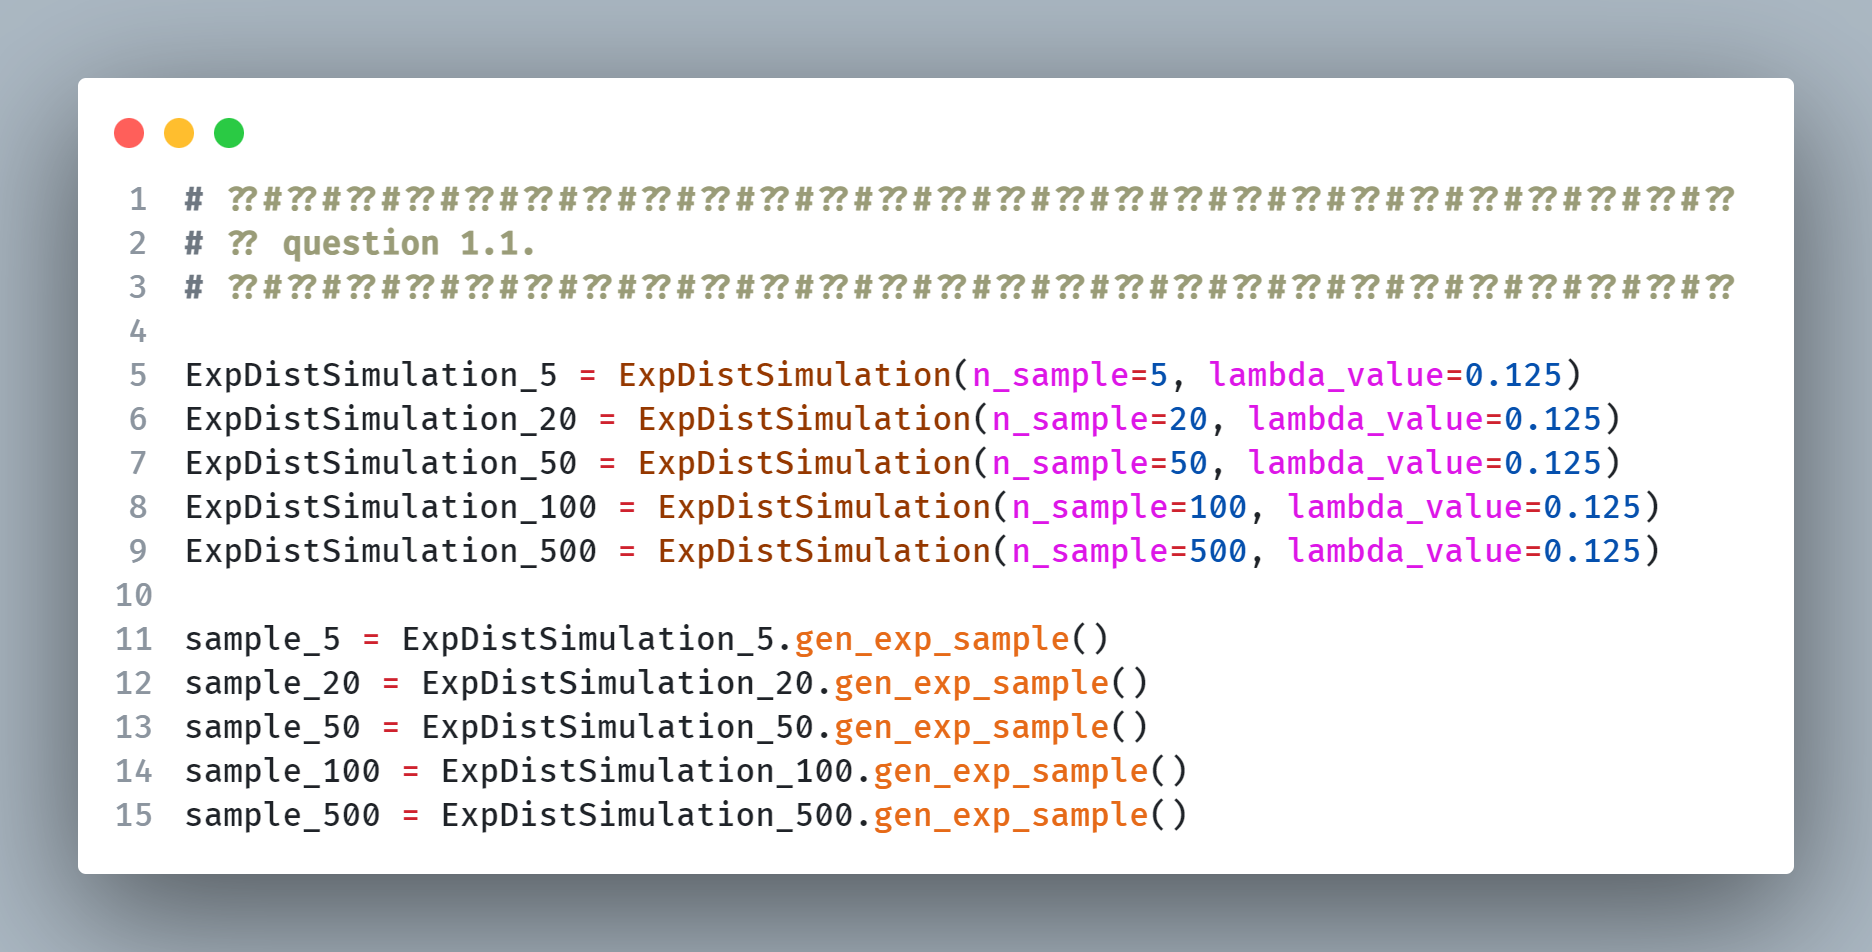
\includegraphics{q1.1.png}}
        \label{q1_1}
    \end{center}
\end{figure}

\begin{figure}[H]
    \noindent\caption{Output for Question 1.1.}
    \begin{center}
        \resizebox{1\textwidth}{!}{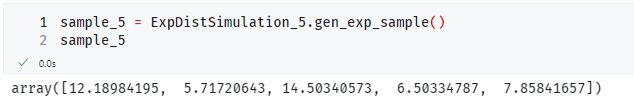
\includegraphics{r1.1.png}}
        \label{r1_1}
    \end{center}
\end{figure}

\subsection{Question 1.2.}

The codes for answering this question are in Figure \ref{q1_2}. Again, for the $n = 5$ case, the raw sample mean is $9.354443709511397$.

\begin{figure}[H]
    \noindent\caption{Codes for Question 1.2.}
    \begin{center}
        \resizebox{1\textwidth}{!}{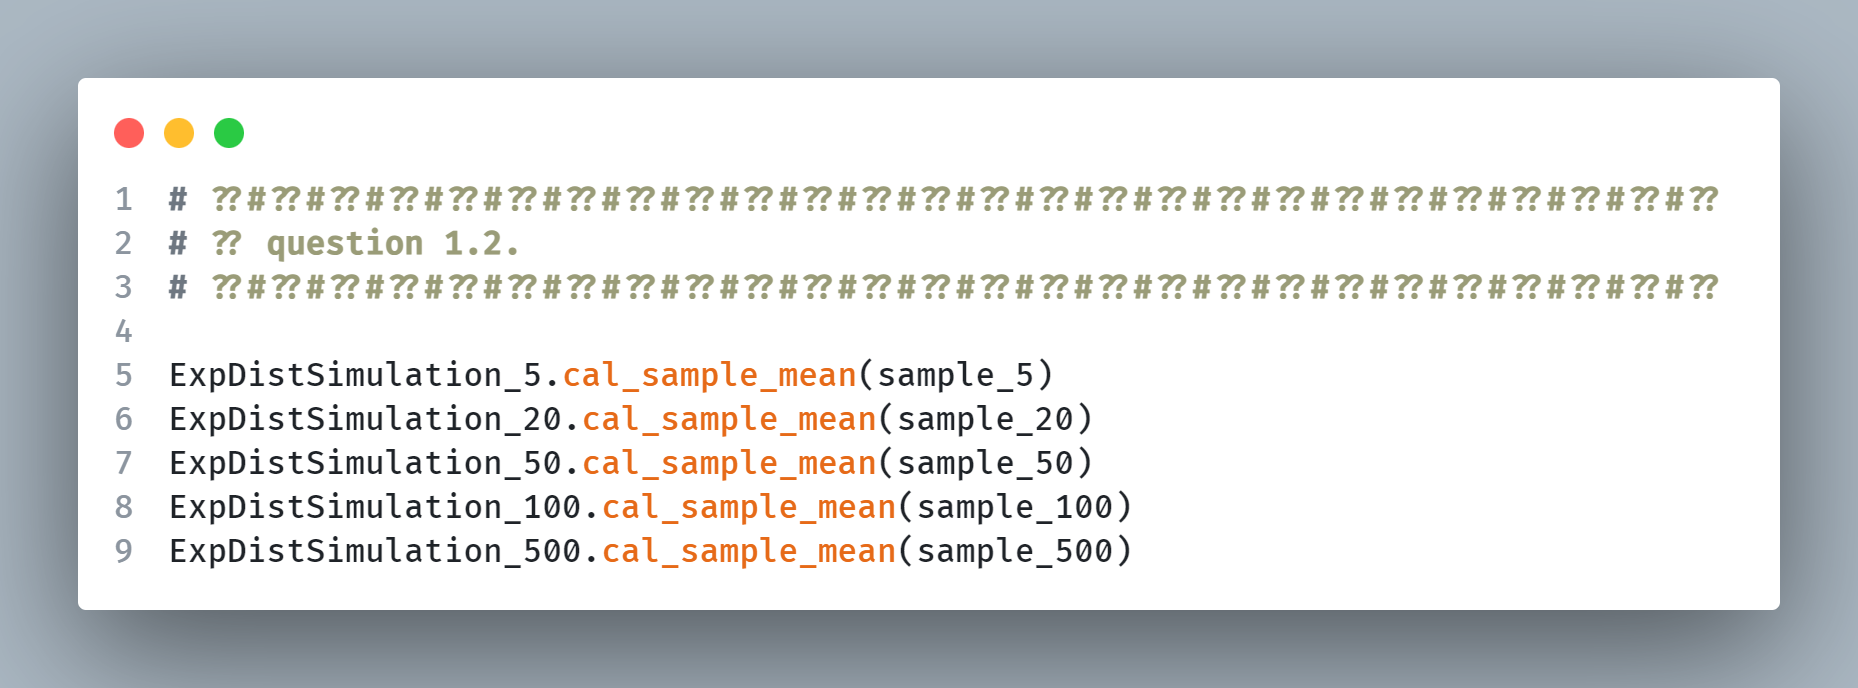
\includegraphics{q1.2.png}}
        \label{q1_2}
    \end{center}
\end{figure}

\subsection{Question 1.3.}

The codes for answering this question are in Figure \ref{q1_3}. Again, for the $n = 5$ case, the adjusted sample mean is $3.0286282061644623$.

\begin{figure}[H]
    \noindent\caption{Codes for Question 1.3.}
    \begin{center}
        \resizebox{0.9\textwidth}{!}{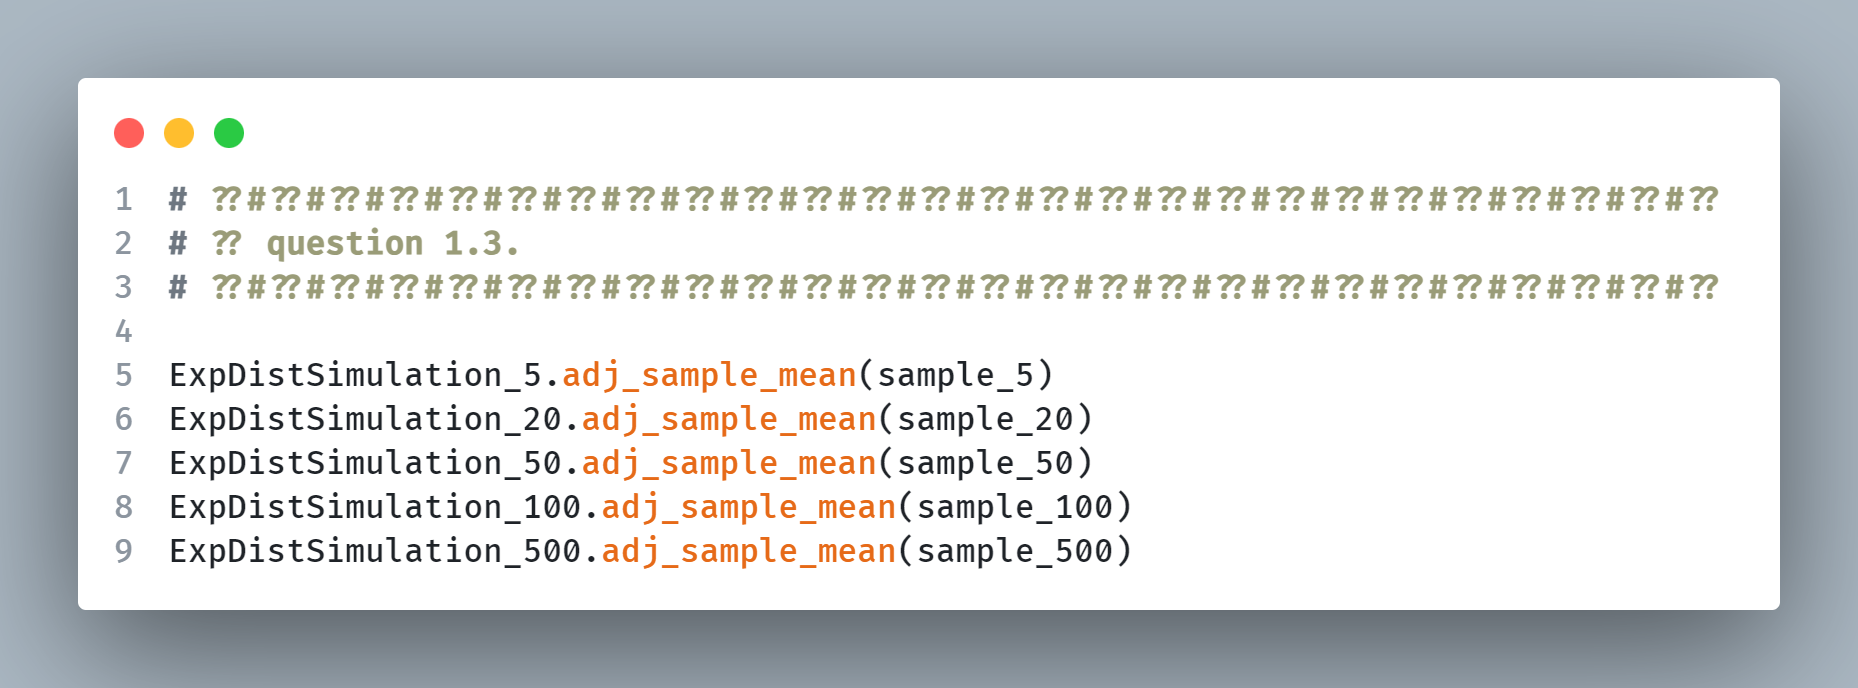
\includegraphics{q1.3.png}}
        \label{q1_3}
    \end{center}
\end{figure}

\subsection{Question 1.4.}

Next, I repeat the procedures in question 1.1.-1.3. for $1000$ times, and plots the empirical distribution of the simulated adjusted means. 

The results are in Figure \ref{dist_adj_means}.

Comments: First, we should expect these adjusted means across different simulated samples should have a normal distribution if the sample size in each simulation sample goes to infinity, as the Central Limit Theorem suggests. It is clear that the empirical distributions become more similar to a normal distribution, as $n$, the sample size in each simulation increases. For example, the $n=5$ case is obviously left-skewed and have a fat right tail, but these properties almost vanish for the $n = 500$ case. This is because the Central Limit Theorem states the asymptotic properties of our statistic of interest, and the asymptotic distribution holds only if we draw enough sample points from the distribution. 

\begin{figure}[H]
    \setcounter{subfigure}{0}
	\noindent\caption{Distribution of the simulated adjusted means with different sample sizes}
	\centering	
	\subfloat[$n = 5$]  {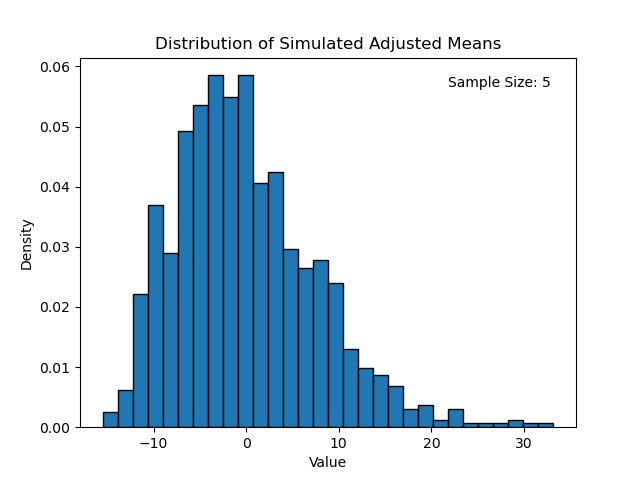
\includegraphics[width=0.48\textwidth]{../results/SimulatedAdjMeans_SampleSize5.png} }
	\subfloat[$n = 20$]  {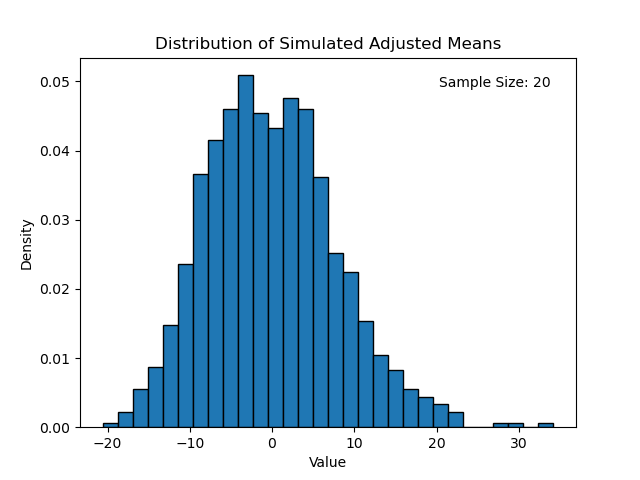
\includegraphics[width=0.48\textwidth]{../results/SimulatedAdjMeans_SampleSize20.png} } \\

    \subfloat[$n = 50$]  {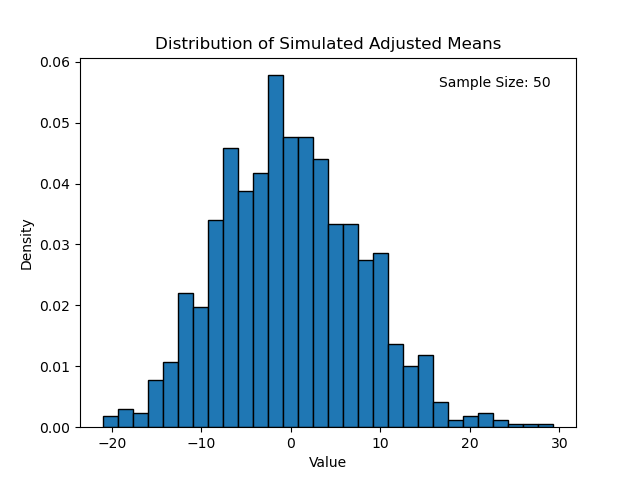
\includegraphics[width=0.48\textwidth]{../results/SimulatedAdjMeans_SampleSize50.png} }
	\subfloat[$n = 100$]  {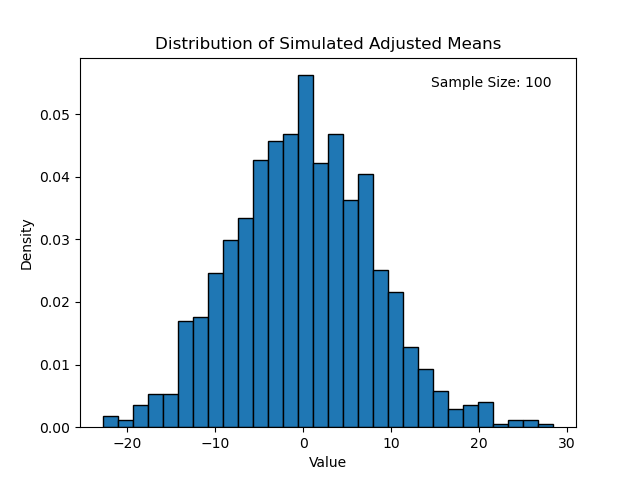
\includegraphics[width=0.48\textwidth]{../results/SimulatedAdjMeans_SampleSize100.png} } \\

    \subfloat[$n = 500$]  {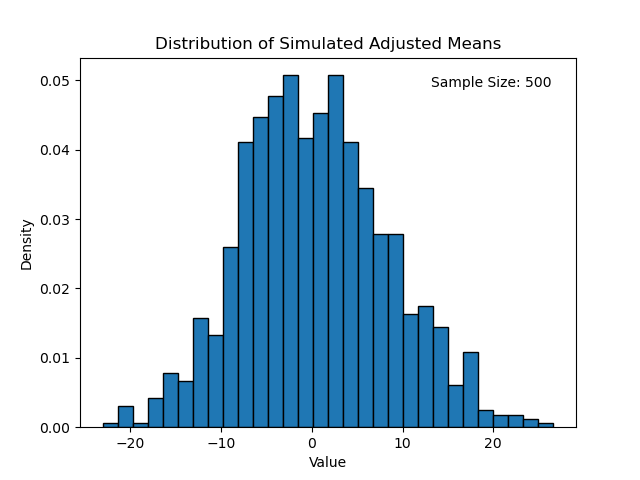
\includegraphics[width=0.48\textwidth]{../results/SimulatedAdjMeans_SampleSize500.png} }
    \label{dist_adj_means}
\end{figure}

\subsection{Question 1.5.}

I guess this question is about MLE, thus the moment condition shouldn't be 
$$
5000 \cdot \log\of{\l} - \l \sum_{i=1}^{5000}x_i = 0.
$$
\highlightP{I use the following optimization problem for estimating the $\l$}:
$$
\max_{\l} \bs{5000 \cdot \log\of{\l} - \l \sum_{i=1}^{5000}x_i}.
$$

In particular, I first create a sample with $5000$ random draws, then define the objective function (which is the negative log-likelihood, since I use a minimization routine), as shown in Figure \ref{q1_5}.

\begin{figure}[H]
    \noindent\caption{Codes for Question 1.5.}
    \begin{center}
        \resizebox{0.7\textwidth}{!}{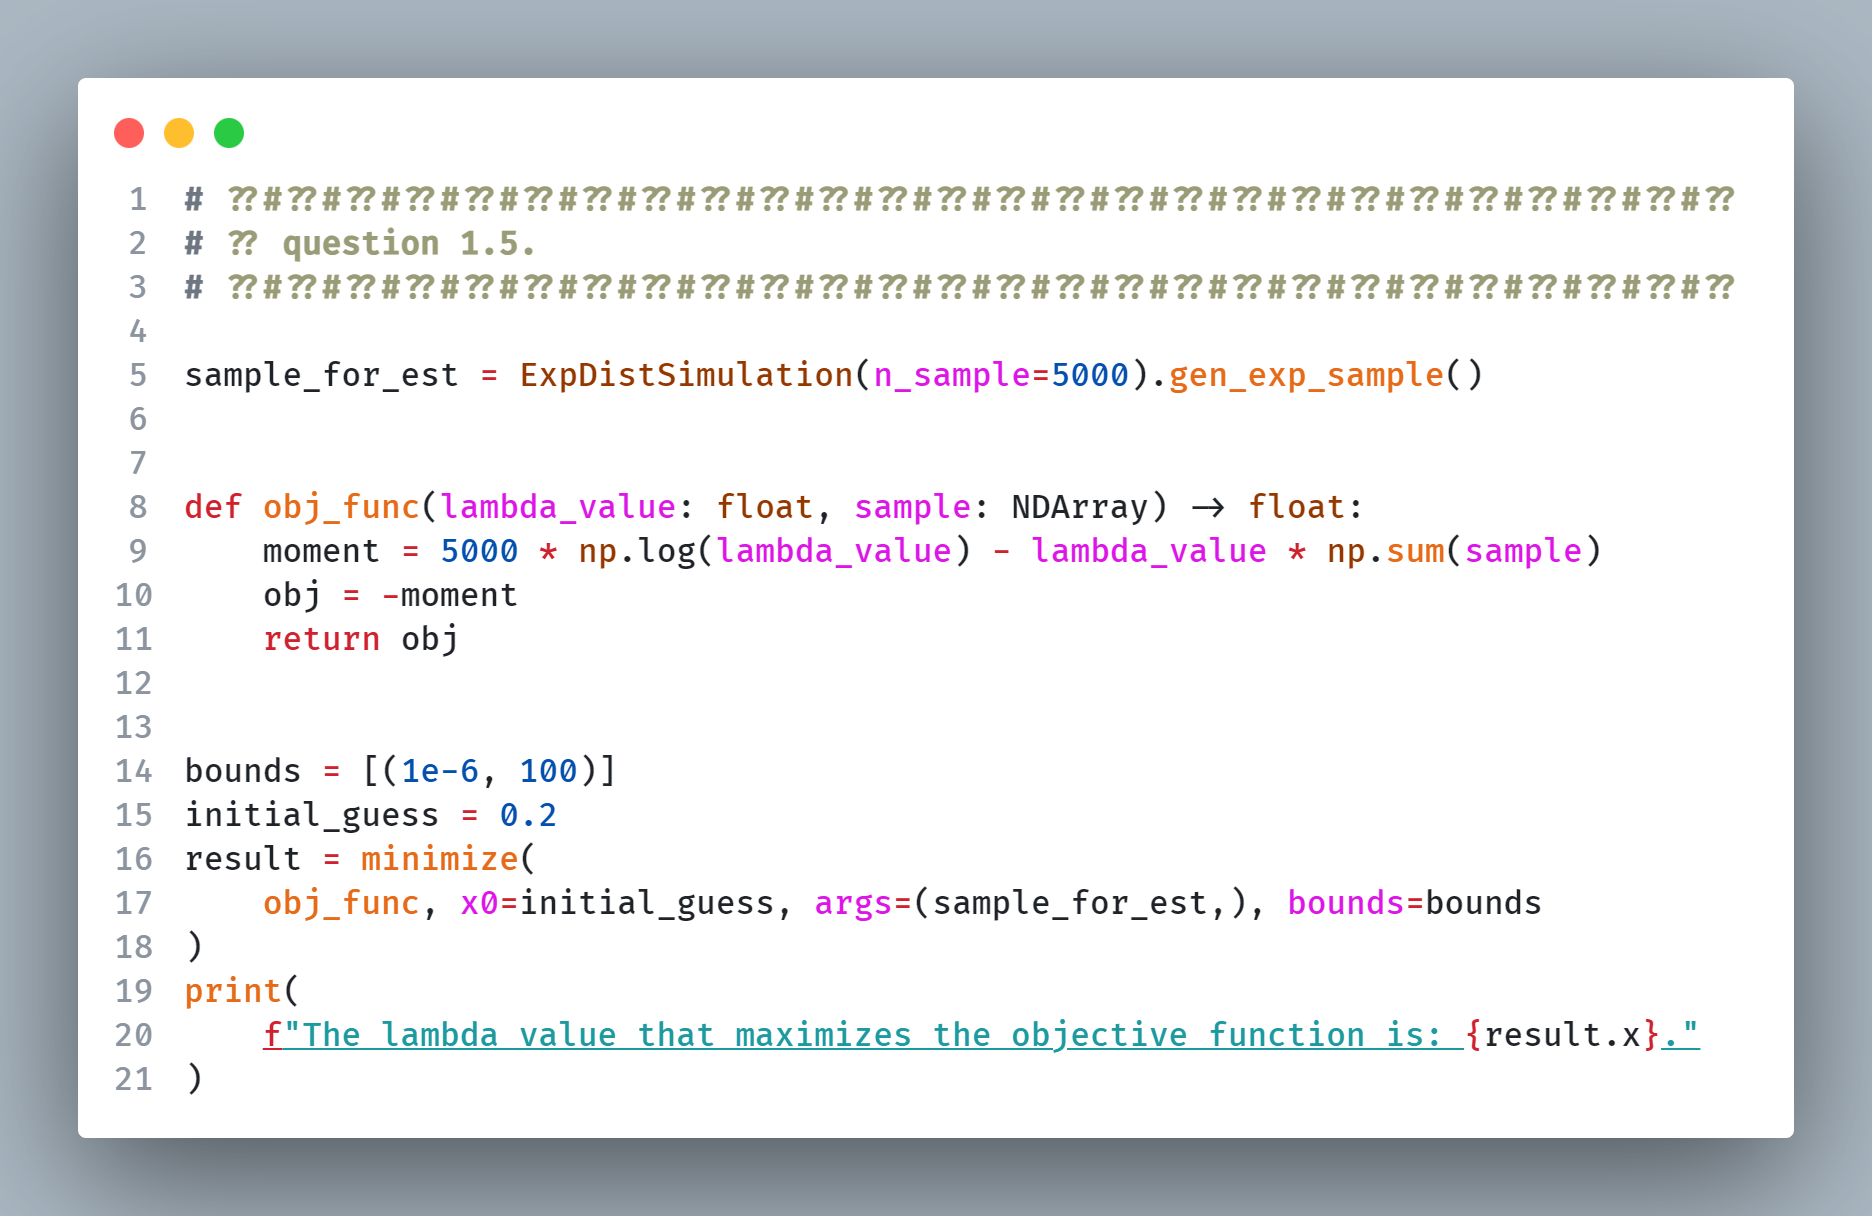
\includegraphics{q1.5.png}}
        \label{q1_5}
    \end{center}
\end{figure}

The results (togher with the codes screenshot) are in Figure \ref{r1_5}. The estimated $\lambda$, $\wh{\l}$ is 0.123. 

\begin{figure}[H]
    \noindent\caption{Answer for Question 1.5.}
    \begin{center}
        \resizebox{0.8\textwidth}{!}{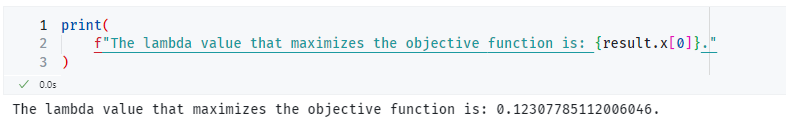
\includegraphics{r1.5.png}}
        \label{r1_5}
    \end{center}
\end{figure}

\subsection{Question 1.6.}

When restricting the search over intervals $\bs{0.5, 1}$ and $\bs{0.2,1}$, the optimizer value is $0.5$, and $0.2$, respectively. These boundary values suggest that the maximization solution in these two cases fail to reach the true maximization (which can be calculated by the first-order condition). Therefore, we need to extend these narrow bound conditions when conducting the numerical maximization. 

But when the restriction is $\bs{0.1, 1}$, we can reach the true optimizer: $0.123$, since we have extended our bound condition to a broader interval.

\subsection{Question 1.7.}

To answer this question, I create a equi-distanced grid over $\bs{10^{-6}, 100}$ as different initial values to start the search, and then for each initial value, I conduct the optimization routine, and stores the results in an array, and plots the results against different starting values. The codes are presented in Figure \ref{codes_1_7}, and the results are in Figure \ref{r1_7}.

\begin{figure}[H]
    \noindent\caption{Codes for Question 1.7.}
    \begin{center}
        \resizebox{0.8\textwidth}{!}{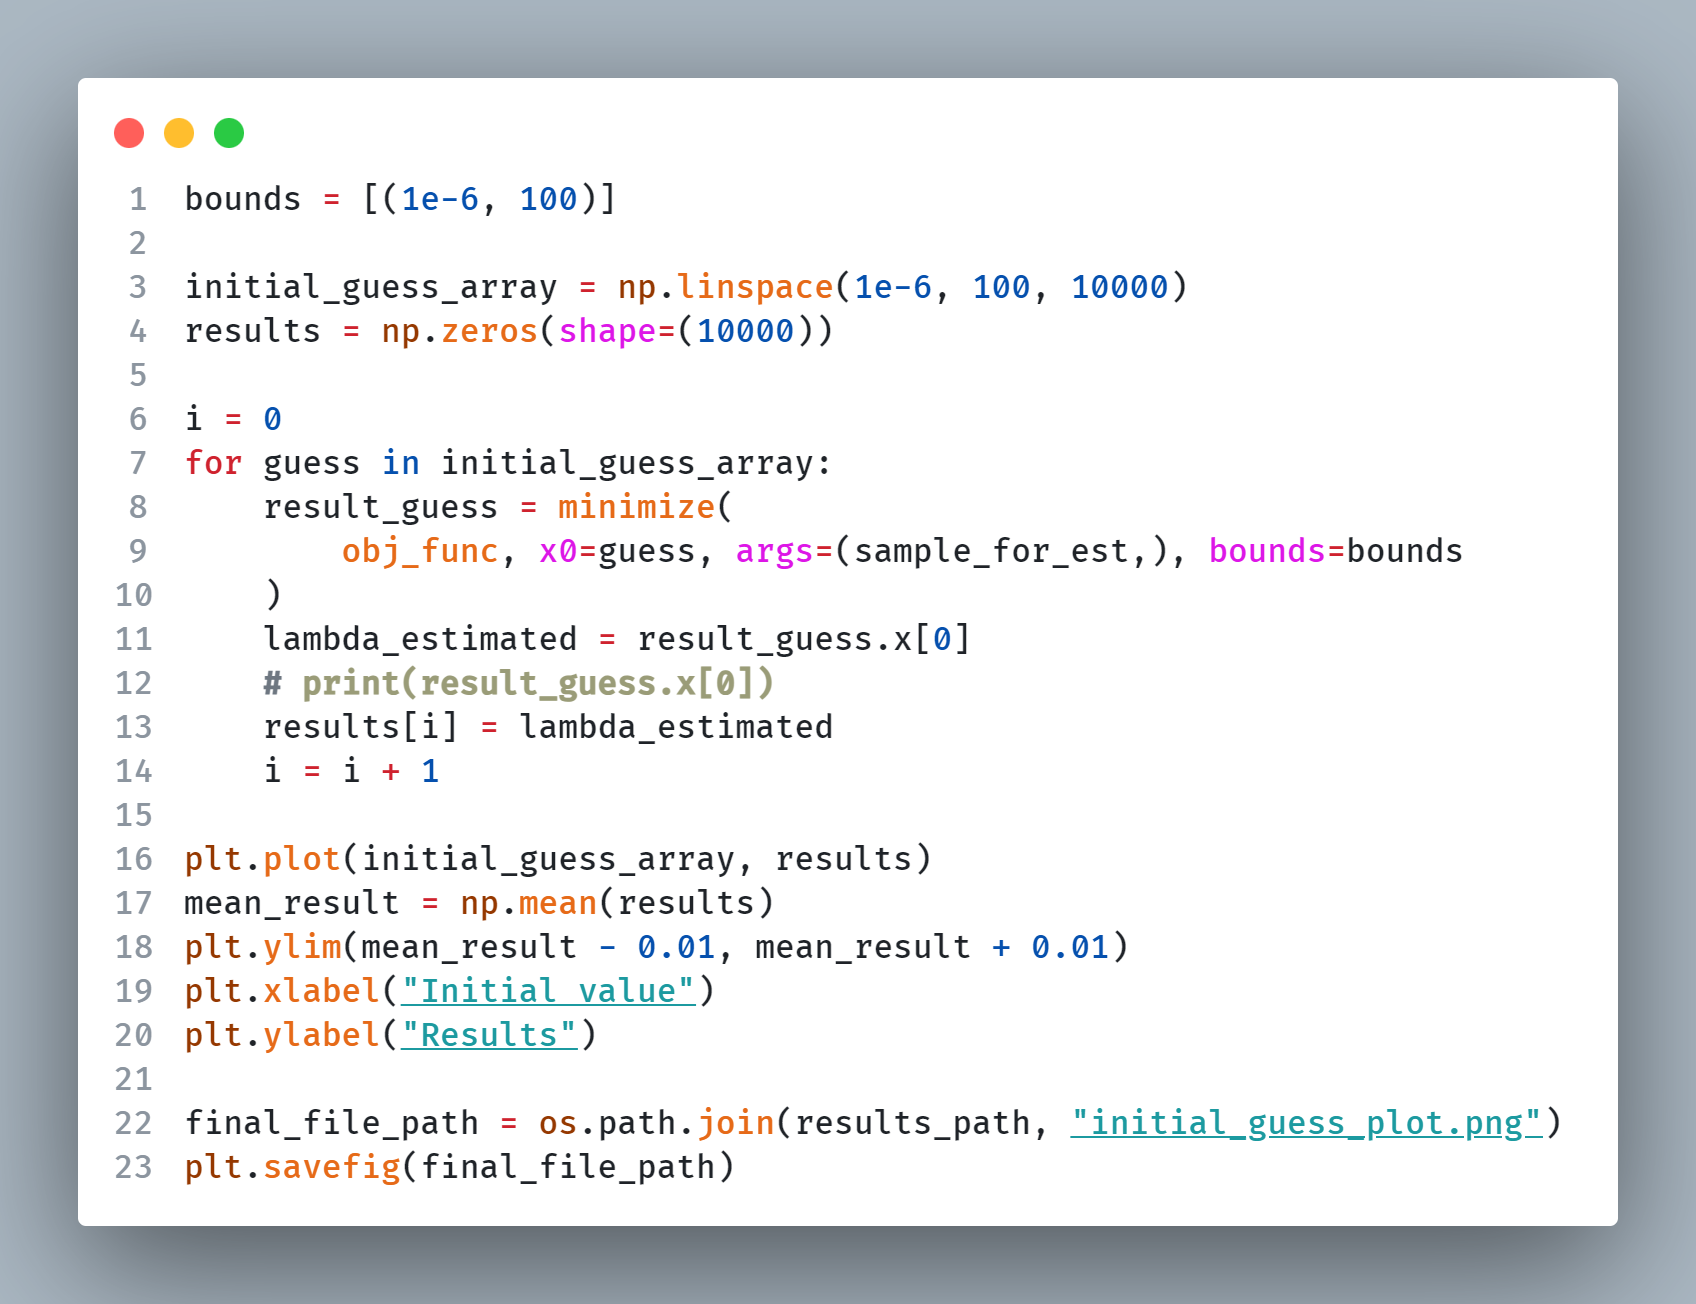
\includegraphics{r1.7.png}}
        \label{codes_1_7}
    \end{center}
\end{figure}
 

\begin{figure}[H]
    \noindent\caption{Answer for Question 1.7.}
    \begin{center}
        \resizebox{0.5\textwidth}{!}{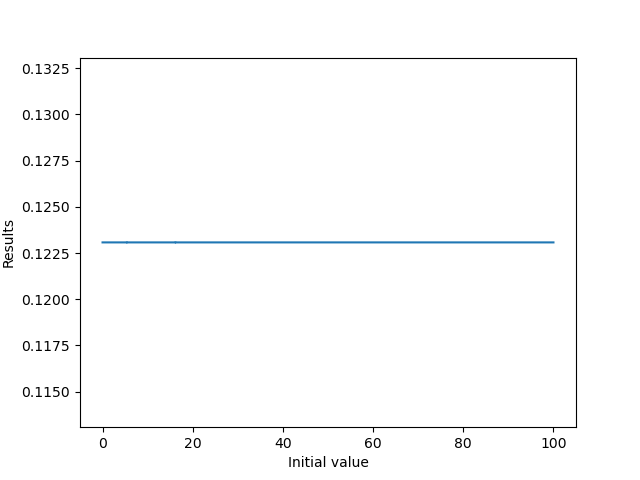
\includegraphics{../results/initial_guess_plot.png}}
        \label{r1_7}
    \end{center}
\end{figure}

It is easy to see that the starting guess values doesn't matter for this MLE problem.

To see the tiny difference between different starting points, we can rescale the y-axis and have the following graph - Figure \ref{r1_7_rescaling}. Notice that the scale of the y-axis is $10^{-6}$!

\begin{figure}[H]
    \noindent\caption{Answer for Question 1.7. - Rescaling the y-axis}
    \begin{center}
        \resizebox{0.5\textwidth}{!}{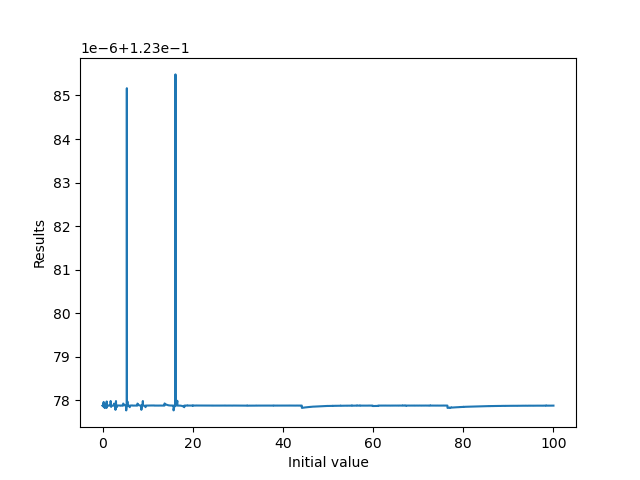
\includegraphics{../results/initial_guess_plot_rescaling.png}}
        \label{r1_7_rescaling}
    \end{center}
\end{figure}

\section{Estimation}

Appendix Figure \ref{Codes_statasetup} stores some Stata commands for initial setup, such as codes for defining several path macros, and specifying the version. The corresponding do file is ``codes/Question2.do''.

\setcounter{subsection}{1}
\subsection{Dataset Construction}

The Stata codes for this question are in Figure \ref{q2_2}. The required moments are 
\begin{itemize}[topsep=0pt, leftmargin=20pt, itemsep=0pt]
\setlength{\parskip}{10pt} 
\item Mean: 311065.
\item Standard deviation: 3193502.
\item P10: 2.597.
\item P50: 1161.257.
\item P90: 2346.26.
\item Number of observations: 28803.
\end{itemize}

\begin{figure}[H]
    \noindent\caption{Codes for Question 2.2.}
    \begin{center}
        \resizebox{0.8\textwidth}{!}{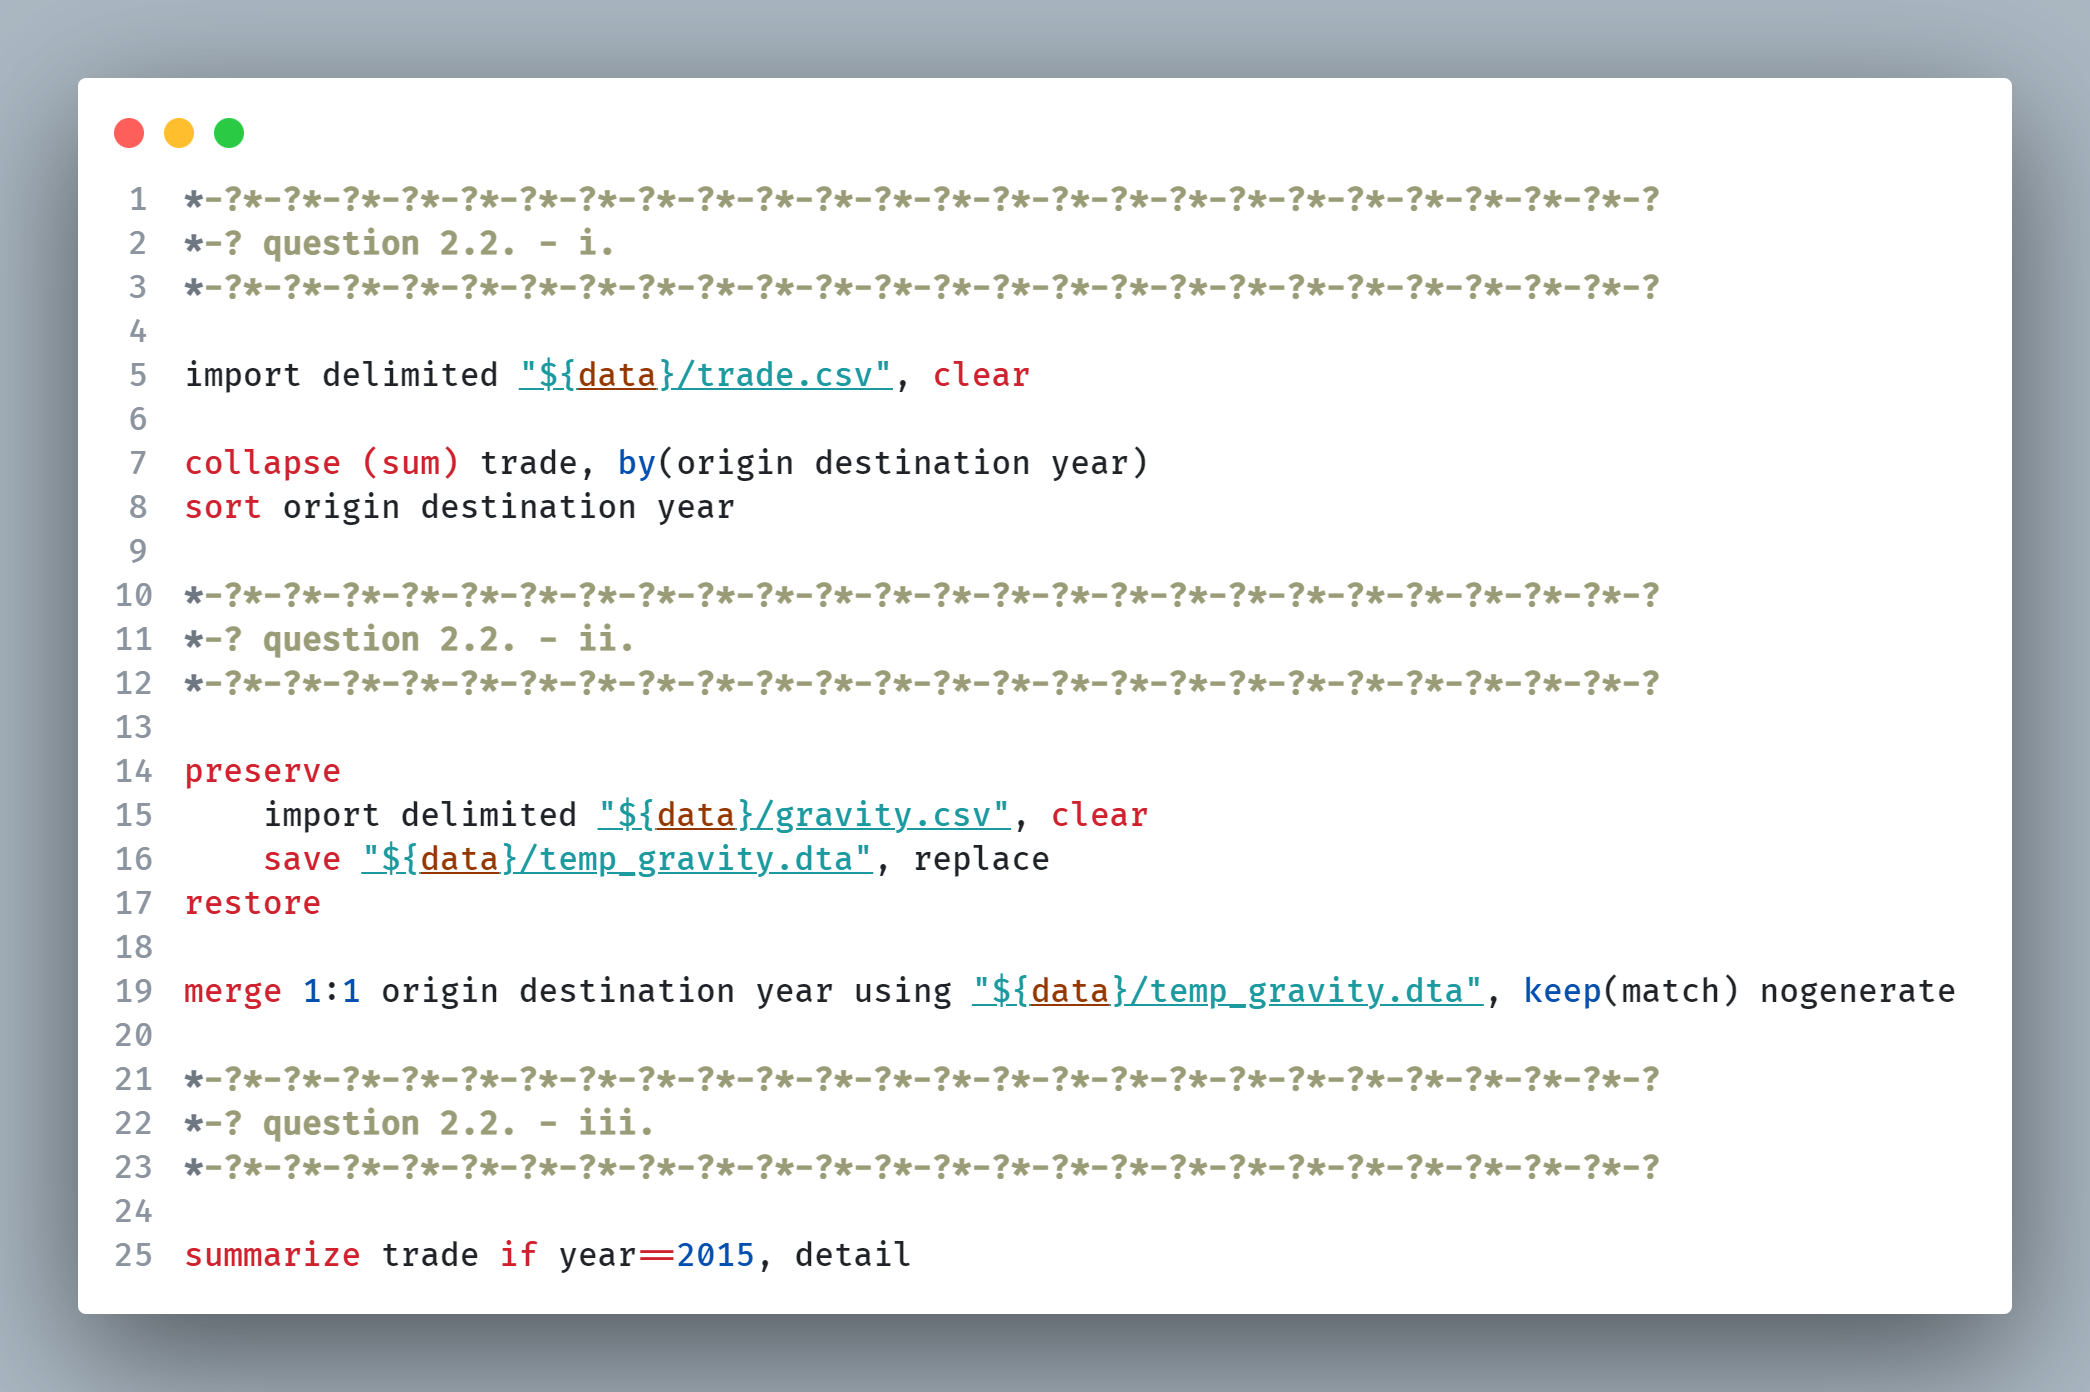
\includegraphics{q2.2.png}}
        \label{q2_2}
    \end{center}
\end{figure}

\subsection{Estimation}

\subsubsection{The Binscatter Plot}

The binscatter plot is in Figure \ref{r2_3_1}. The raw correlation between log(trade flows) and log(distance) is $-0.2608$. The linear fit (with a constant) of the regression coefficient on  log(distance) is $-1.396478$.

\begin{figure}[H]
    \noindent\caption{Binscatter plot of trade flows against distance}
    \begin{center}
        \resizebox{0.9\textwidth}{!}{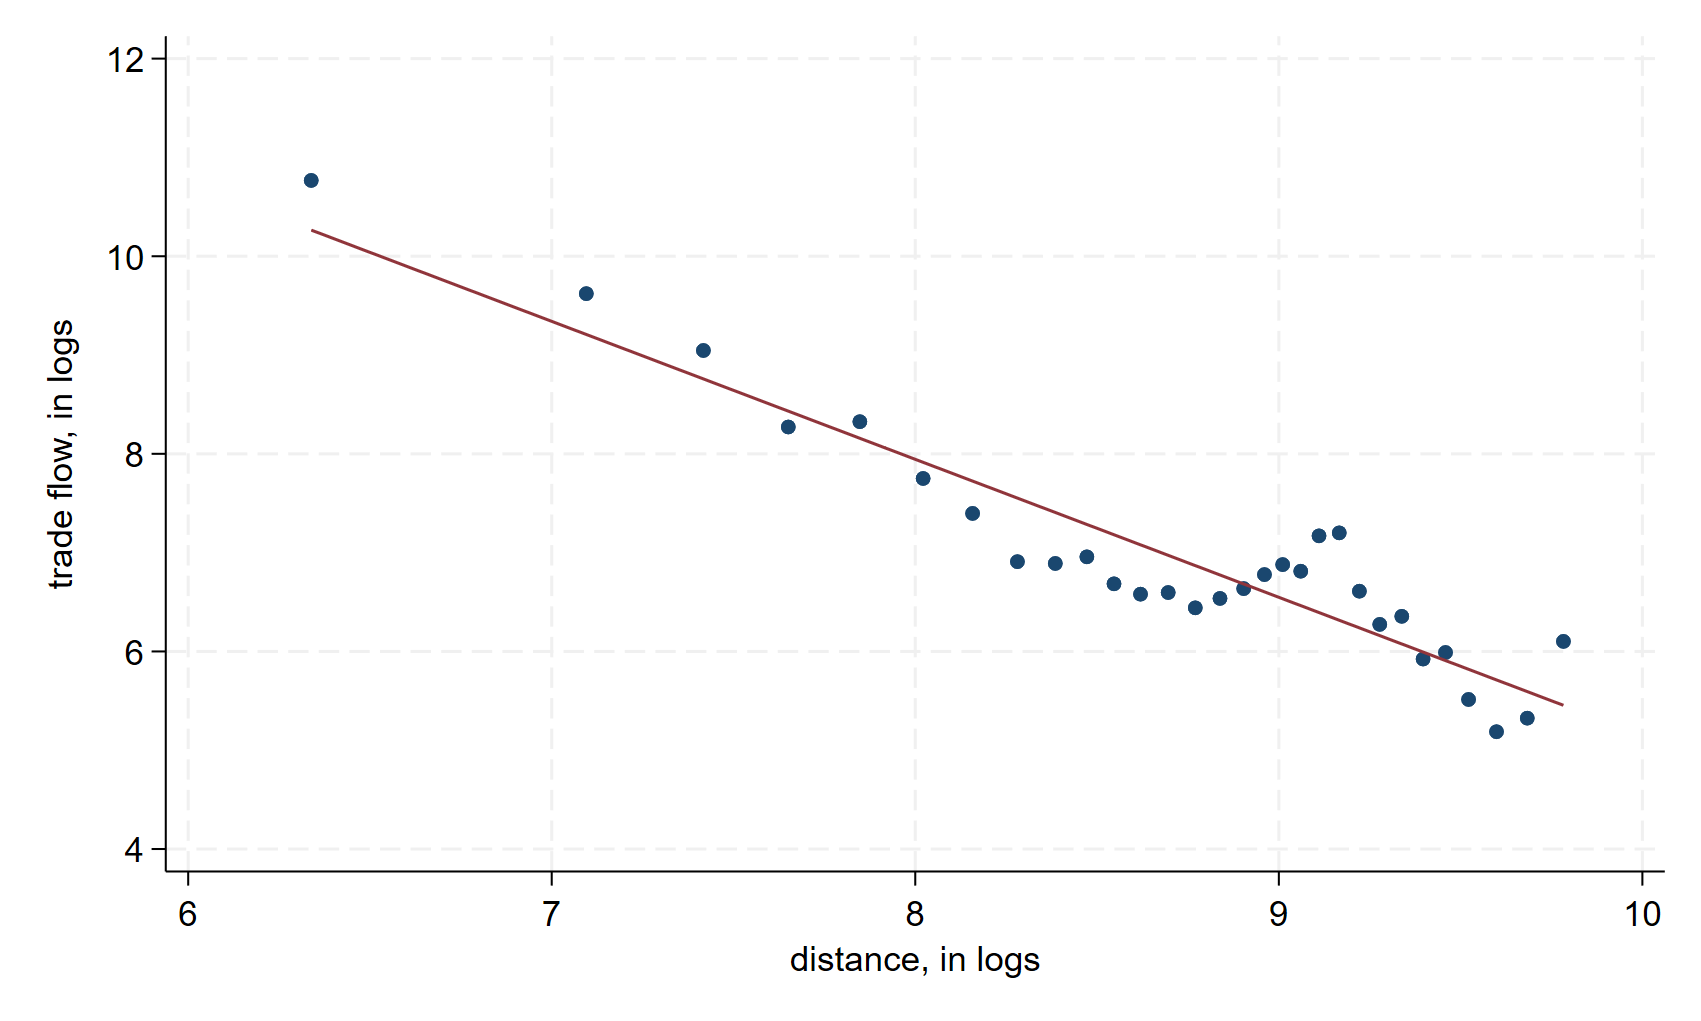
\includegraphics{../results/binscatter_trade_distance.png}}
        \label{r2_3_1}
    \end{center}
\end{figure}

\newpage 
\subsubsection{Distance Coefficients Across Years}

The results are in Figure \ref{r2_3_2}. In the graph, I report the estimated coefficients using sample from different years, and the 95\% confidence intervals, which are calculated based on clustered standard errors (two-way clustering on both the origin and the destination countries).

\begin{figure}[H]
    \noindent\caption{Coefficients on log(distance) for different years}
    \begin{center}
        \resizebox{0.9\textwidth}{!}{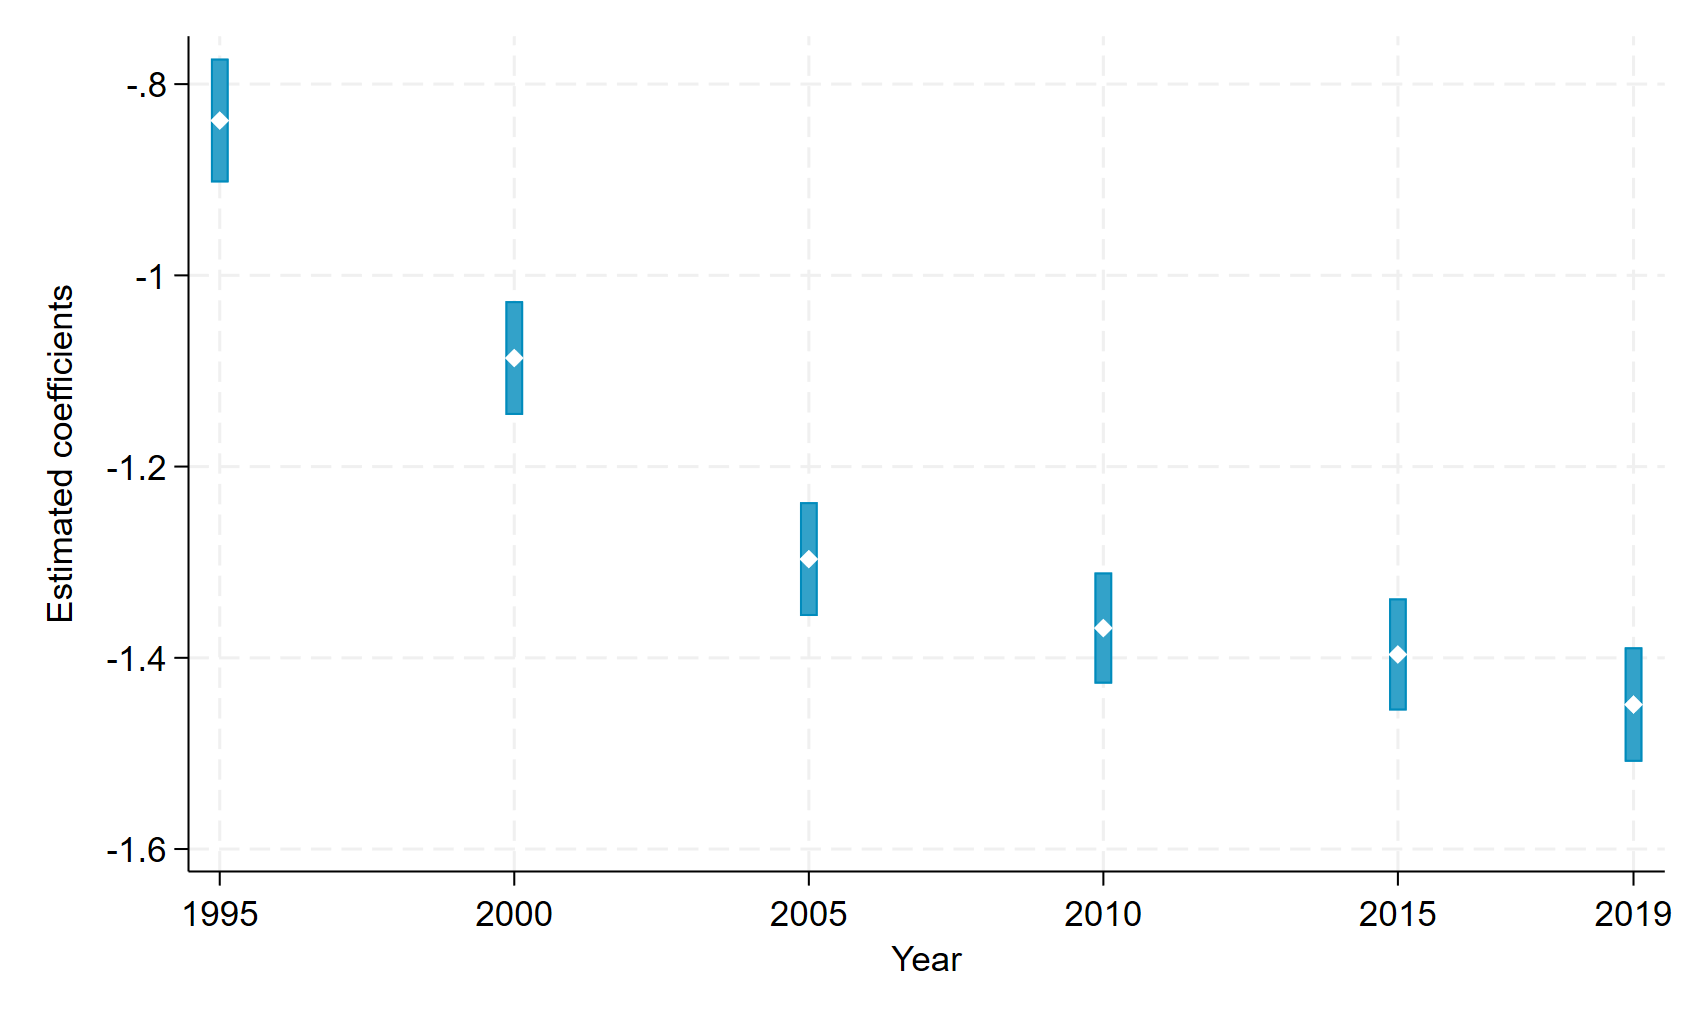
\includegraphics{../results/DistanceCoeffAcrossYears_Cluster.png}}
        \label{r2_3_2}
    \end{center}
\end{figure}

\newpage 
\subsubsection{Distance Coefficients Across Years With Importer and Exporter FEs}

The results are in Figure \ref{r2_3_3}, where the estimated coefficients using sample from different years, and the 95\% confidence intervals, which are calculated based on robust standard errors are reported.


\begin{figure}[H]
    \noindent\caption{Coefficients on log(distance) for different years, with importer-year and exporter-year FEs}
    \begin{center}
        \resizebox{0.9\textwidth}{!}{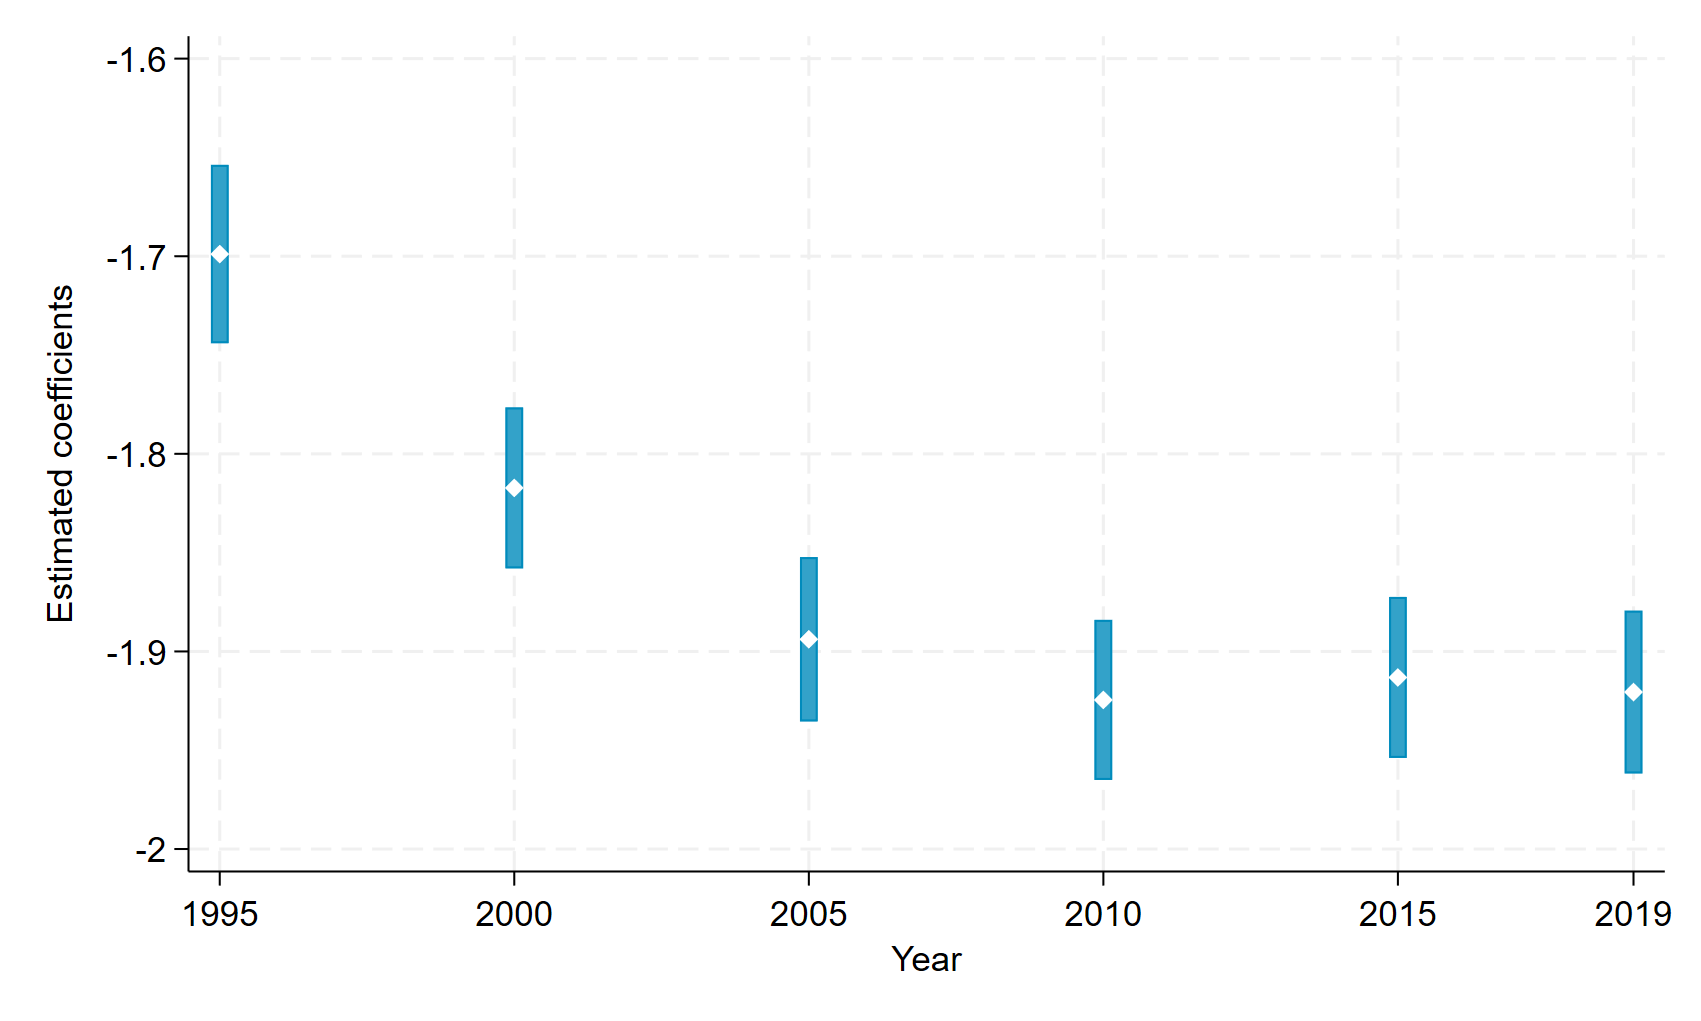
\includegraphics{../results/DistanceCoeffAcrossYears_FE.png}}
        \label{r2_3_3}
    \end{center}
\end{figure}

Discussion:

In Figure \ref{r2_3_3}, where importer-year and exporter-year FEs are controlled, we are essentially reporting how much percentage of trade flows will decrease between two given countries in a given year, if their distance has increased by 1\%. Controlling for importer and exported fixed effects allow us to partial out the effects of some country attributes, such as economy size (e.g., as measured by GDP) from the estimated coefficients. However, in Figure \ref{r2_3_2}, where the FEs are not controlled, the variation used to identify the distance coefficient could also come from different importer-exporter pair with different distance. 

\newpage 
\subsubsection{Adding Other Controls}

The required table is Table \ref{regressiontable}, where the robust standard errors are reported in parentheses. 

\begin{table}[H]
	\centering
	\caption{}
    \resizebox{0.5\textwidth}{!}{
        \begin{threeparttable}
            \def\sym#1{\ifmmode^{#1}\else\(^{#1}\)\fi}
\begin{tabular}{lc}
\toprule
\toprule
& \multicolumn{1}{c}{Trade flows} \\ 
                    &\multicolumn{1}{c}{(1)}         \\
\hline
distance, in logs   &      -1.588\sym{***}\\
                    &      (0.02)         \\
[1em]
sharing a border    &       1.100\sym{***}\\
                    &      (0.10)         \\
[1em]
sharing a language  &       1.008\sym{***}\\
                    &      (0.05)         \\
[1em]
having colonial ties&       0.558\sym{***}\\
                    &      (0.12)         \\
[1em]
having a trade agreement&       0.555\sym{***}\\
                    &      (0.04)         \\
\hline
R-squared           &       0.724         \\
Obs                 &       26938         \\
\hline
\hline
\end{tabular}
\begin{tablenotes}
\footnotesize
\item
Notes. Sample includes trade flows between different countries in 2015. Importer and exporter fixed effects are controlled. Robust standard error are reported. 
\end{tablenotes}

        \end{threeparttable}
    }
	\label{regressiontable}
\end{table}

Discussion:

In the table, the coefficient on distance is essentially reporting how much percentage of trade flows will decrease between two given countries who don't share a border, or a language, or colonial ties, and don't have a trade agreement in a given year, if their distance has increased by 1\%. Compared with Figure \ref{r2_3_3}, the effect of distance on the trade flows between two countries decreases when we add more controls that represent other notions of ``distance'' between two countries. The decrease is most likely due to the fact that these controls (especially ``sharing a border'') are negatively correlated with the geographical distance measure. 

All other controls measure the easiness for trades to happen between different countries. In particular, ``sharing a border'' measures geographical distance, ``sharing a language'' and ``sharing colonial ties'' measures some type of cultural linkages, and ``having a trade agreement'' measures some institutional costs for international trade. For instance, if two countries share the same language, then it is easier for importer firms to communicate with the exporter firms -- they are more likely to match each, negotiate with each other and reach a business contract. Therefore, it is intuitive that these factors will contribute positively to trade flows between two countries. 


\appendix 

\section{Appendix}

\setcounter{figure}{0}
\renewcommand{\thefigure}{A.\arabic{figure}}

\begin{figure}[H]
    \noindent\caption{}
    \begin{center}
        \resizebox{0.45\textwidth}{!}{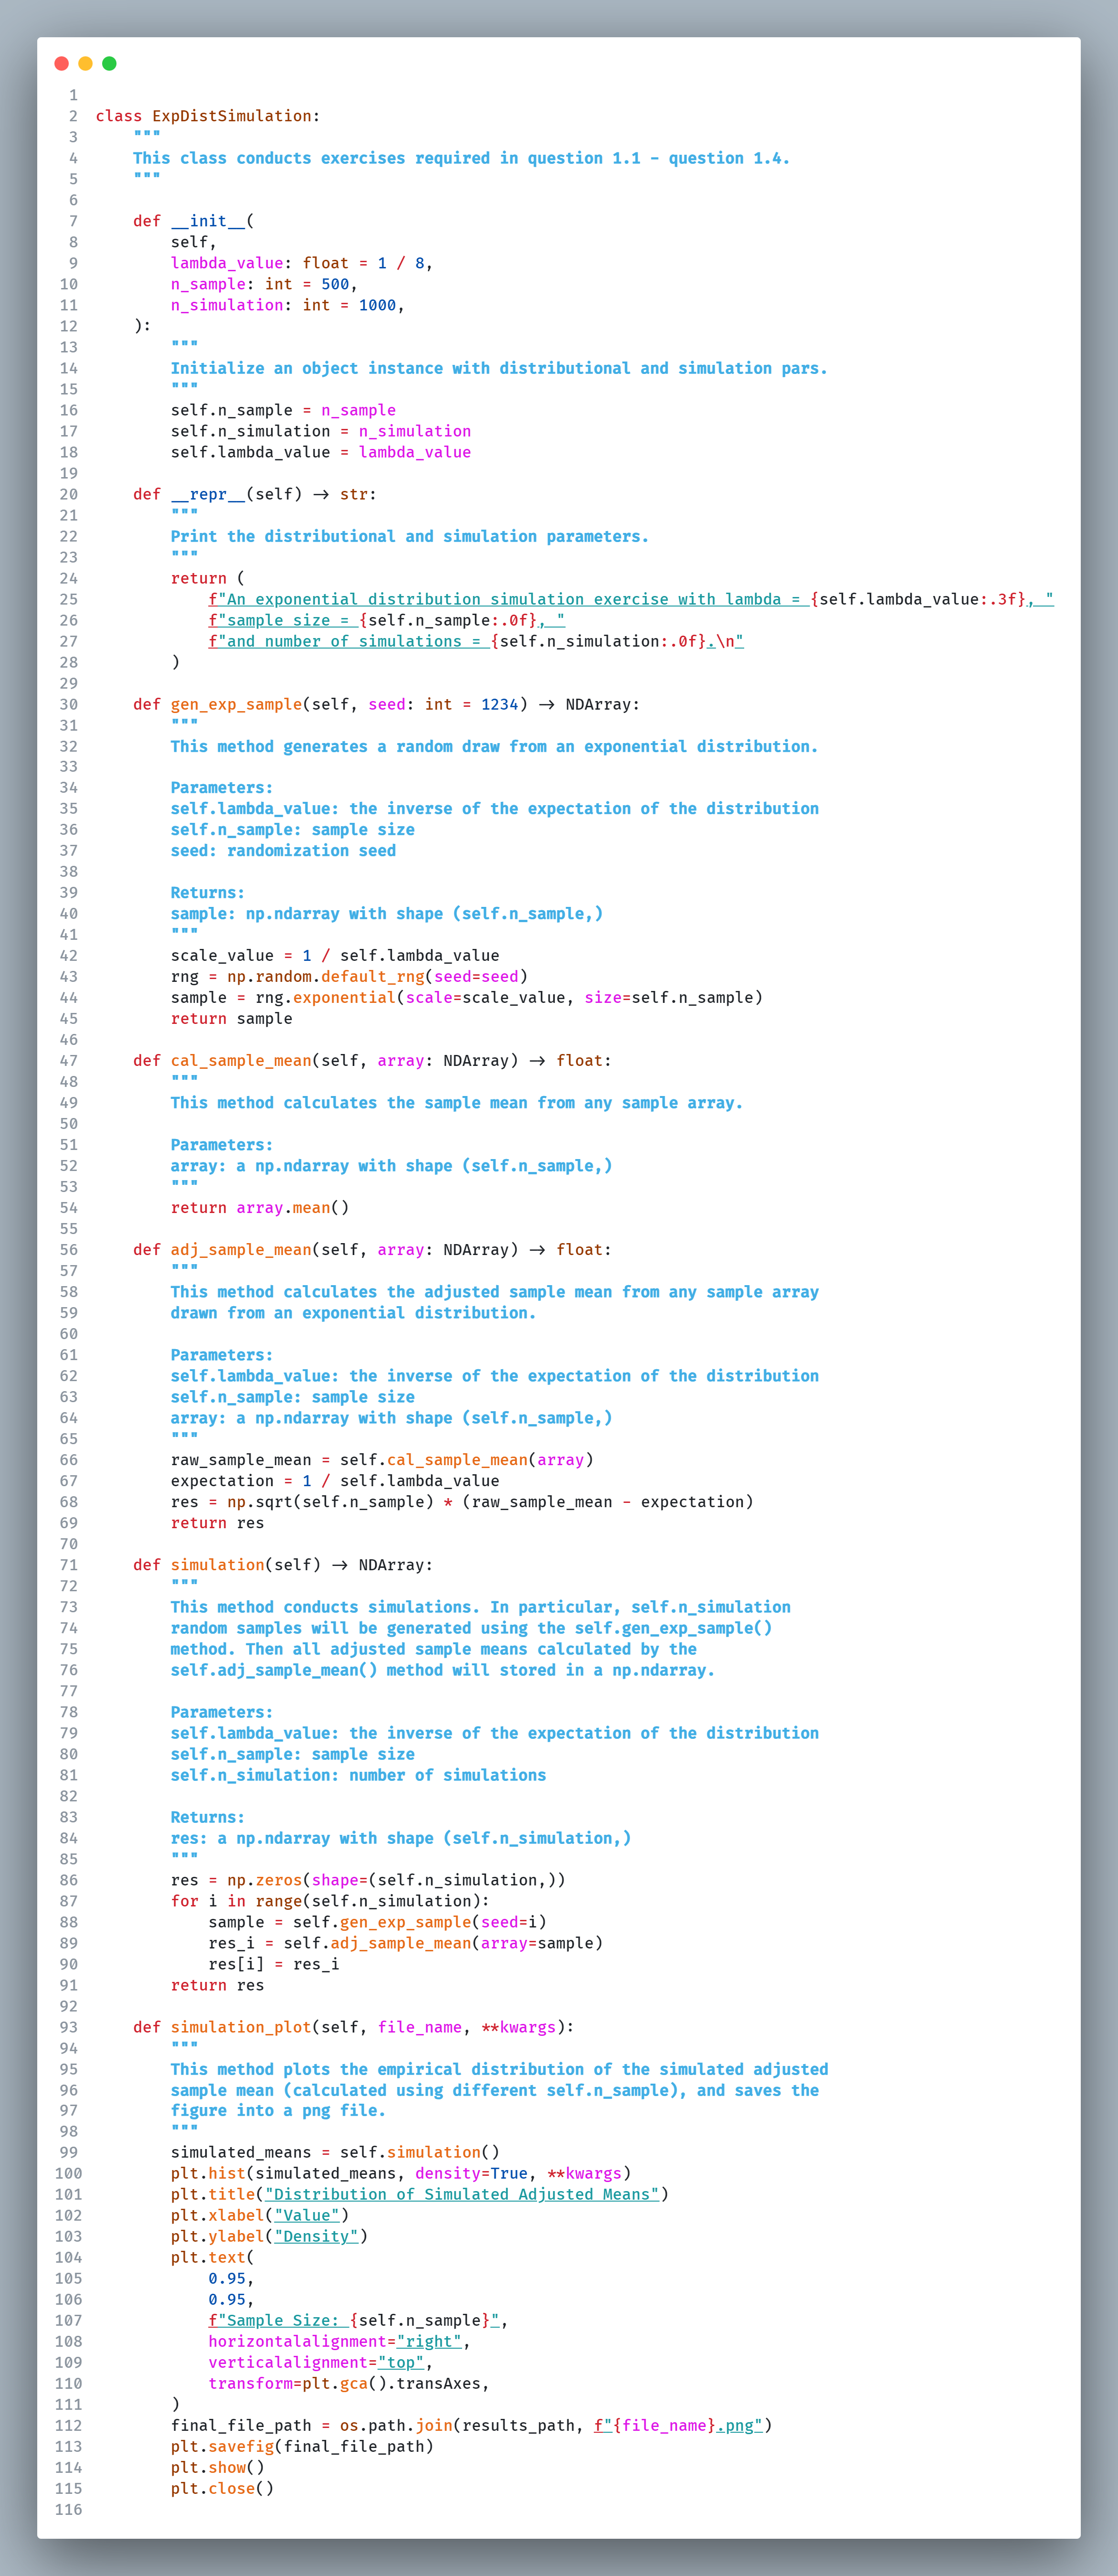
\includegraphics{Codes_class.png}}
        \label{Codes_class}
    \end{center}
\end{figure}

\begin{figure}[H]
    \noindent\caption{}
    \begin{center}
        \resizebox{1\textwidth}{!}{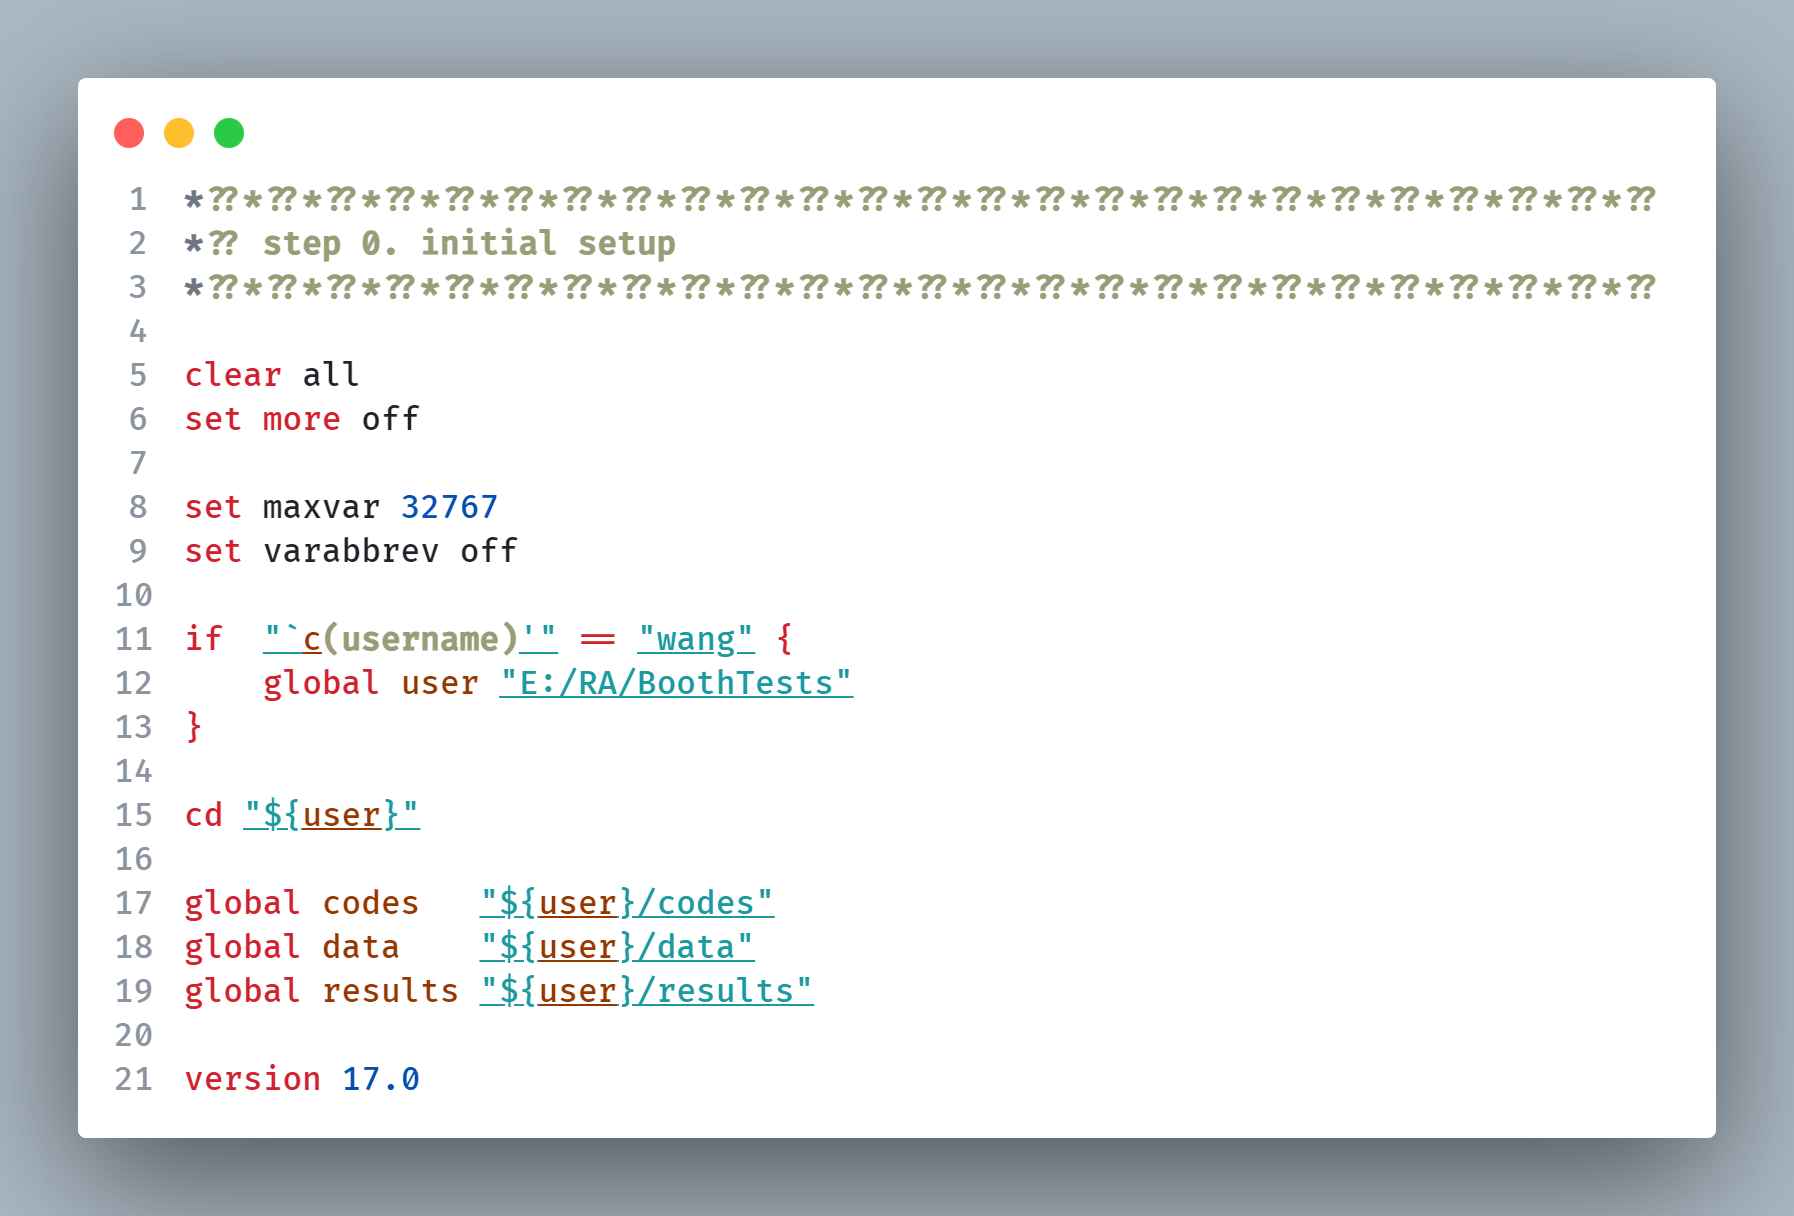
\includegraphics{Codes_statasetup.png}}
        \label{Codes_statasetup}
    \end{center}
\end{figure}

\end{document}